\documentclass[a4paper,twoside, onecolumn]{IEEEtran}
\title{Bachelor thesis by Tim Budweg} 
\author{}
\date{11.03.2015}

\usepackage{amsthm}
\usepackage{graphicx}
\graphicspath{{figures/eps/}}


\newtheorem{lemma}{Lemma}[section]
\newtheorem{prop}{Proposition}[section]
\newtheorem{definition}{Definition}[section]
\begin{document}
\maketitle

\section{Introduction}
Wireless ad-hoc sensor networks are very useful. 
You can create warning systems for emergency purposes.
For instance, deploying many sensor nodes into the sea or forest to check and caution for tsunamis or fire.
Another use case is
\section{Algorithm}
\section{Reactive construction}
\section{Proof}
The authors of \cite{kanj} use $LDel^{(2)}(U) $ as the underlying subgraph of the Modified Yao Step.
$LDel^{(2)}(U) $ is defined as the subgraph of U in which the circumcircle of every triangle does not contain a 2-hop-neighbor of the nodes which create the triangle.
However, it is not known whether $LDel^{(2)}(U) $ can be constructed reactively.
At this point I want to introduce the \emph{Partial Delaunay Triangulation (PDT)} \cite{pdt} which might be a valid replacement.
The following part of this work will examine the possibility of this replacement.

At first, note that the style of this proof is adapted from \cite{kanj}.
Let U be the Unit Disk Graph of the Euclidean Graph of a Node Set S.
In a style similar to the definition of $LDel^{(2)}(U) $ from \cite{kanj}, we define the Partial Delaunay Triangulation as follows:
\begin{definition}
\label{emptycircle}
An edge XY of U is contained in the PDT graph if and only if there exists a circle trough X and Y whose interior contains no point of U that is a 2-hop neighbor of X or Y.
\end{definition}
This can be verified since the original PTD-Definition from \cite{pdt} is defined like above, except that the circle must not contain \emph{any} nodes of U. 
If this region contains no nodes at all, it cannot contain nodes which are 2-hop-neighbors of X or Y either.  

Additionally, the following Delaunay Graph property is being used:
\begin{lemma}
\label{emptyregion}
If CA and CB are edges of the PDT Graph then the region of $(O)=\bigcirc{ABC} $ subtended by chord  CA and away from B and the region of $(O) $ subtended by chord CB and away from A contain no points that are two hop neighbours of A, B and C.
\end{lemma}


See Figure \ref{fig:empty_region} for a graphical illustration of the above lemma.
This property also holds true for PDT.

\begin{proof}
Since $CA $ is a PDT edge there is a circle $c_1 $ with C and A on it's border which does not contain any node (or at least non two-hop-neighbour of C or A) of U.
Suppose we take another third Point D, which is not in the Set U, to identify the circle $c_1 $.
No matter where the third point D of this circle is, the region, in the following named $R_1 $, of $\bigcirc{ABC} $ delimited by chord $CA $ away from B is always contained completely in the circle $c_1 $ and, therefore, empty.
By symmetry of circles it is sufficient to put D on a line  $l $ which is defined as the median line of $CA $. 
There are two possibilities on which D can be located. %check located at?
First, D is contained in the Gabriel Graph.
If D moves away from B crossing $CA $ we get the same circles as D moves to B away from $M_{CA} $.
If D crosses B, B is contained in the circle, hence $CA $ cannot be a PTD edge. This is a contradiction to the precondition.
If D is barely in the triangle near $M_{CA} $, $R_1 $ is contained in $\bigcirc{ABC} $.
If D is barely in the triangle near $B $, $R_1 $ is also contained in $\bigcirc{ABC} $.

\end{proof} 


With this lemma in hand Keil and Gutwin ref proved the existence of a path between the Points $A $ and $B $ in the region $R_1 $.
\begin{figure}[h!]
\centering
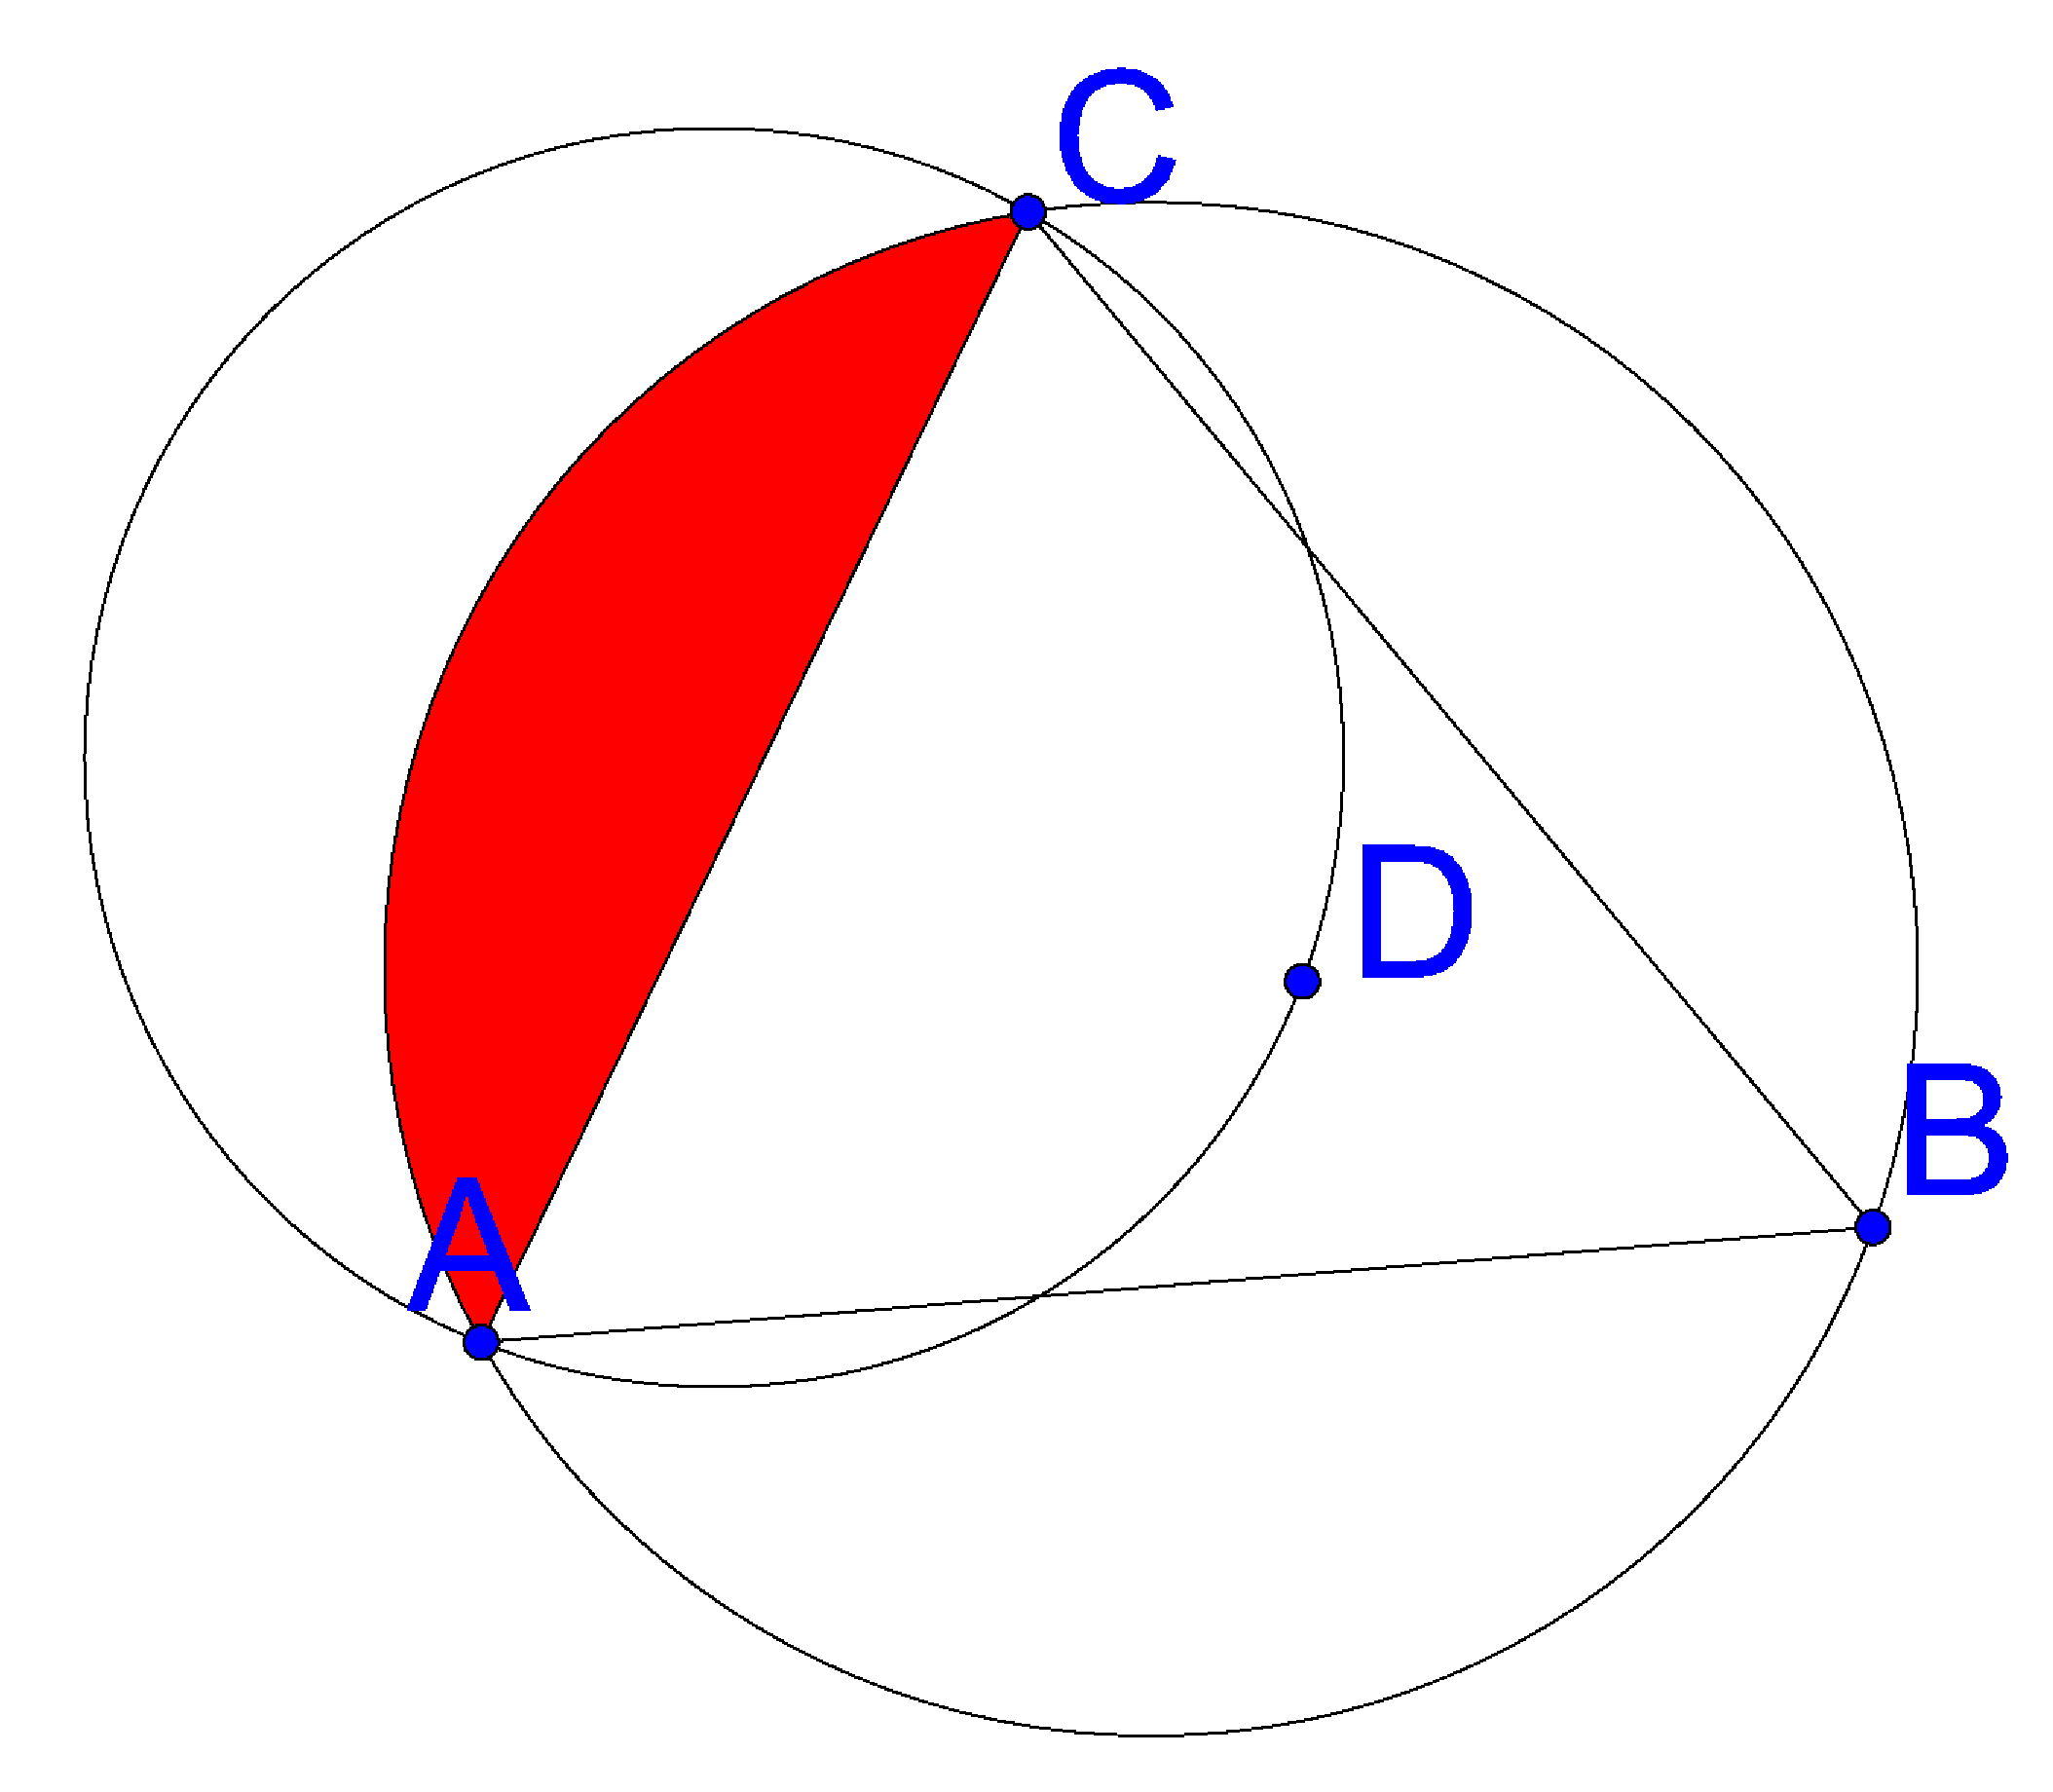
\includegraphics[width=0.2\linewidth]{noPointinRegion.eps}
\caption{The red marked region contains no Points of G because it is always contained in $\bigcirc{ACD} $ which must be empty by definition.}
\label{fig:empty_region}
\end{figure}


We need to show that the inward and outward path are still valid for PDT.
To do so, we must proof these properties:
\begin{enumerate}
\item $|CA| + \sum\nolimits_{i=0}^{r-1} |M_iM_{i+1}| \leq (1+2\pi (k*\cos{\frac{\pi}{k}})^{-1})|CB| $
\item There is no edge in G between any pair $M_i $ and $M_j $ lying in the closed region delimited by CA, CB and the edges of p, for any i and j satisfying $0 \leq i < j-1 \leq r $ 
\item $\angle{M_{i-1}M_iM_{i+1}} > \frac{k-2}{k}\pi $, for $i=1, ..., r-1 $ 
\item $\angle{CAM_1} \geq \frac{\pi}{2}-\frac{\pi}{k} $
\end{enumerate}







\section{Discussion and Conclusion}

\section{Programming}

\bibliographystyle{IEEEtran}
\bibliography{biblio}
\end{document}